\chapter{Progettazione e architettura}
\label{outline}
Nel momento della progettazione, sono stati prefissati alcuni punti importanti:
il programma avrebbe dovuto essere veloce, modulare e parametrizzabile sulle
caratteristiche pi\`u rilevanti dei segnali. L'utilizzo del \CC come linguaggio di
sviluppo ha portato alla scelta di scrivere preferibilmente codice orientato
agli oggetti e di sfruttare al massimo gli strumenti offerti dalla libreria
boost\footnote{\url{http://www.boost.org/}}, praticamente uno standard per
qualunque programma \CC di una certa complessit\`a.
\section{Obiettivi}
Il funzionamento desiderato per l'applicazione \`e piuttosto semplice: il
programma legge dei dati da una sorgente, li trasforma con una \ac{FFT} ed
eventualmente applica qualche filtro, infine scrive l'output su una qualche
destinazione. Un importante obiettivo \`e che la manipolazione dei segnali
avvenga con elaborazione lossless, cio\`e che le operazioni vengano calcolate
abbastanza velocemente da riuscire ad elaborare i dati man mano che arrivano
dalla sorgente.

Uno degli utilizzi principali ipotizzati per lo spettrometro \`e l'elaborazione
di dati per il progetto \ac{seti}. In questo caso, i dati vengono recuperati da
una speciale scheda di acquisizione dedicata\footnote{L'hardware necessario a
sviluppare questo aspetto dell'applicazione non era disponibile, perci\`o
l'implementazione dell'acquisizione di dati \ac{seti} \`e stata lasciata come
possibile sviluppo futuro. cfr. \ref{seti}}.  Le caratteristiche fondamentali
della \ac{FFT} sono una lunghezza del segnale piuttosto importante (circa
$2^{23}$), un basso numero di integrazioni e la possibilit\`a di ricevere i dati
sporadicamente, cio\`e il data rate pu\`o essere mantenuto basso.

Un'altro utilizzo \`e l'analisi di space debris dove la sorgente di dati sono
dei pacchetti UDP e la \ac{FFT} \`e caratterizzata da segnali di lunghezza contenuta
(circa $2^{15}$) con molte integrazioni (circa $100000$). In questo caso \`e
importante riuscire a mantenere il data rate alto, quindi l'elaborazione deve
essere il pi\`u veloce possibile.

\section{Gerarchia di classi}
Per raggiungere gli obiettivi prefissati, sono necessarie alcune classi per
astrarre alcuni concetti. In particolare ci sono tre componenti fondamentali:
\begin{itemize}
\item Una sorgente da cui prendere dati
\item Filtri o trasformazioni da applicare al segnale
\item Una destinazione su cui scrivere l'output
\end{itemize}
Per questo motivo ci sono tre classi astratte che rappresentano questi tre
concetti, oltre a delle classi utili come contenitori di dati. Insieme
formano le basi su cui viene implementato l'algoritmo rappresentato in
figura \ref{fig:algorithm}.
\begin{figure}[htb]
	\begin{center}
		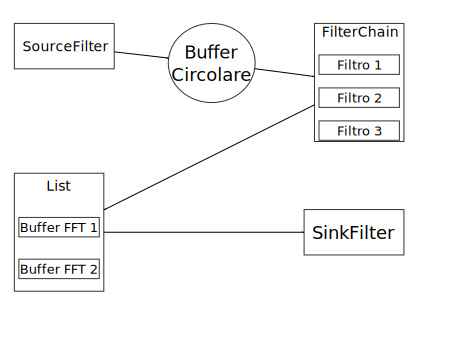
\includegraphics[width=1\linewidth]{algorithm}
	\end{center}
	\caption{Flusso dei dati all'interno del programma}
	\label{fig:algorithm}
\end{figure}

\subsection{SourceFilter}
Una sorgente ha un unico metodo assolutamente necessario che serve a leggere i
dati. Una sottoclasse di \texttt{SourceFilter}, ad esempio, \`e il server UDP
(\texttt{udp\_sock}), che pu\`o essere usata da qualunque codice generico che
faccia riferimento unicamente all'interfaccia astratta. Se si creasse un'altra
sottoclasse di \texttt{SourceFilter} e la si sostituisse a \texttt{udp\_sock} si
otterrebbero i dati da un'altra fonte senza dover cambiare una riga di codice al
di fuori della inizializzazione.
\subsection{ProcessFilter}
Un \texttt{ProcessFilter} rappresenta una qualunque elaborazione intermedia del
segnale, sia essa una trasformata di Fourier o un filtro passa---basso o una
qualunque altra manipolazione. Siccome in questa fase si prende un segnale e lo
si manipola in qualche maniera, l'interfaccia richiede un metodo
\texttt{transform} che abbia in input i dati da elaborare e scriva su un vettore
di output specificato. I filtri sono per natura concatenabili, quindi per
gestire questa coda serve una classe \texttt{FilterChain} che si occupi di
passare l'elaborazione attraverso una coda di filtri precedentemente
selezionati.
\subsection{SinkFilter}
Le destinazioni hanno bisogno di un unico metodo di interfaccia: \texttt{write}.
In modo simile al \texttt{SourceFilter}, una qualunque implementazione della
classe astratta \texttt{SinkFilter} pu\`o essere intercambiata con un'altra
senza dover apportare modifiche al codice, permettendo di scegliere il
dispositivo di memorizzazione pi\`u adeguato agli scopi perseguiti.
\subsection{Contenitori di dati}
Sono state progettate alcune classi al fine di astrarre i dati e assicurarne la
corretta sincronizzazione.
\subsubsection{SrcType}
\texttt{SrcType} \`e una struttura con un costruttore, un destruttore ed un
operatore di assegnamento. Tra i membri di questa struttura c'\`e una mutex per
eseguire operazioni in mutua esclusione, ove necessario. Questa struttura \`e un
wrapper di un puntatore, ideale per essere usata all'interno di un circular
buffer.
\subsubsection{FFTBuf} La classe \texttt{FFTBuf} \`e un vettore su cui
vanno scritti i risultati di una o pi\`u trasformazioni di Fourier. Al momento
della costruzione, si indica la lunghezza del segnale da salvare e il numero di
integrazioni che si prevede di fare; a questa maniera \`e possibile assegnare
questo buffer a tanti thread quante dovranno essere le integrazioni da fare. La
classe offre strumenti anche per tener traccia di quante integrazioni sono già
state effettuate e sapere cos\`i se il buffer \`e pronto per essere scritto su
output.
\subsubsection{List}
La classe \texttt{List} \`e un semplice wrapper attorno ad una lista della
libreria standard. Questa classe assicura un comportamento corretto in ambienti
multithreading e aggiunge alcuni metodi per semplificare la coordinazione con
gli altri thread.

\subsection{Wrapper di librerie}
La classe \texttt{IPP} esiste solo per fornire un wrapper \CC alle librerie
\ac{ipp}, scritte in C. Tramite overloading \`e stato possibile utilizzare lo
stesso nome per funzioni che operano su tipi di dati differenti, lasciando al
compilatore il compito di invocare la funzione specifica pi\`u adeguata.

\section{Threading}
\begin{figure}[htb]
	\begin{center}
		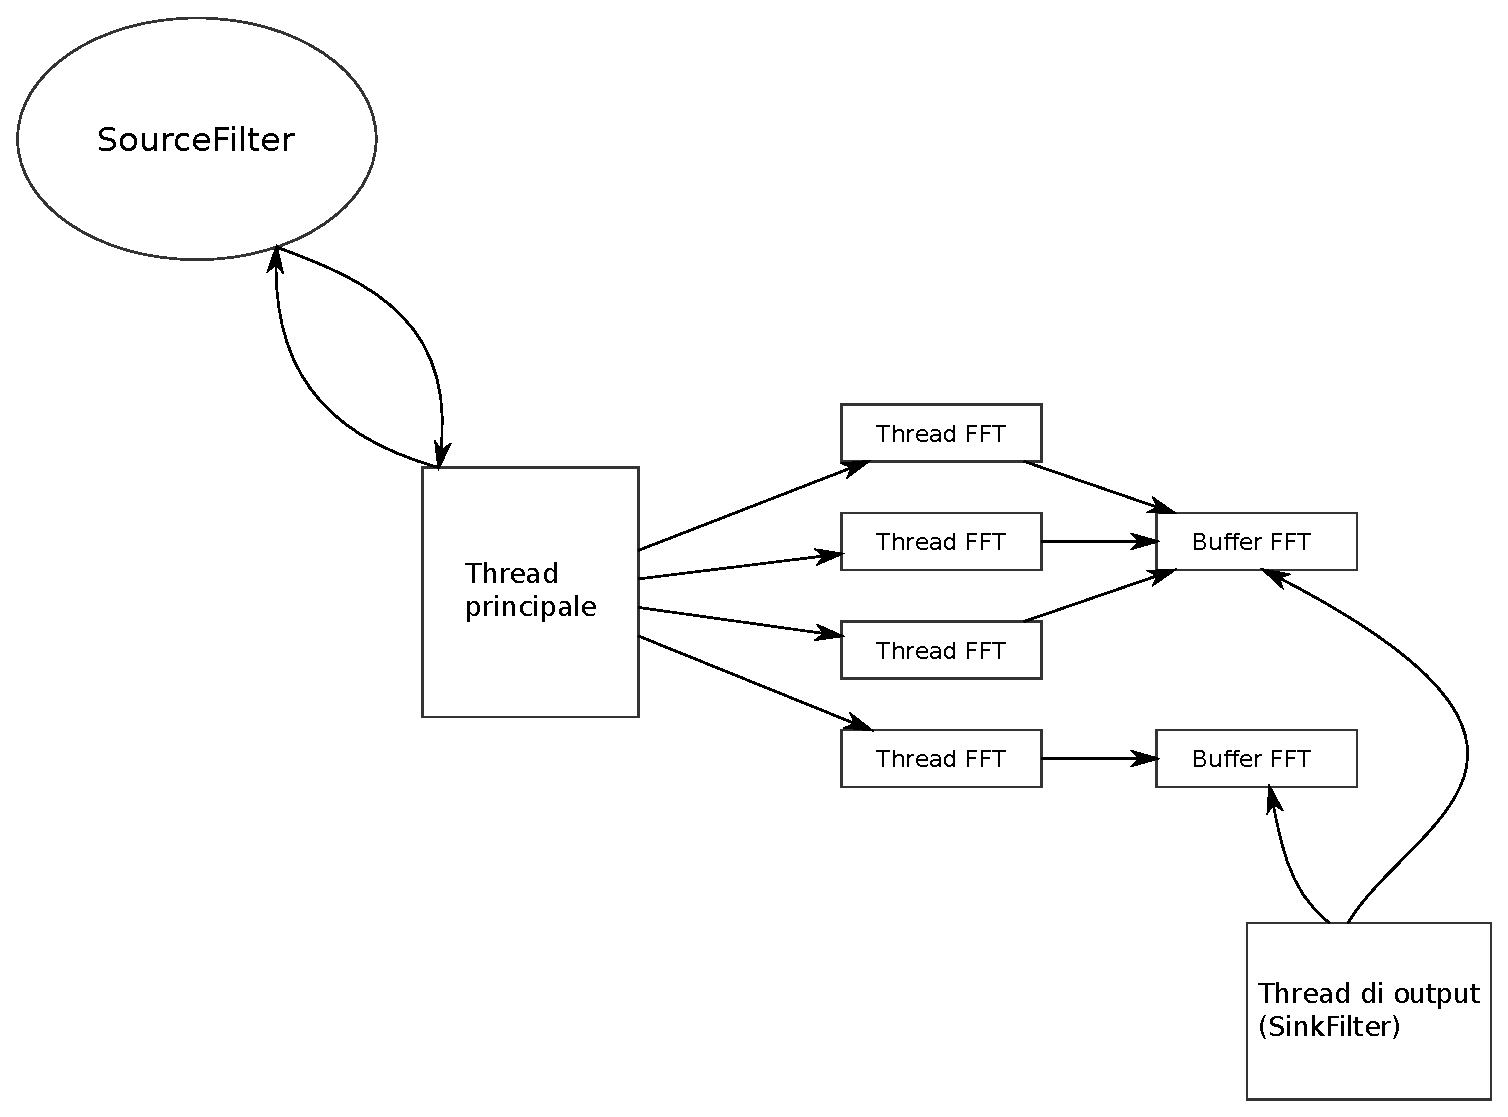
\includegraphics[width=1\linewidth]{threading}
	\end{center}
	\caption{Interazione dei diversi thread tra loro.}
	\label{fig:threading}
\end{figure}
Per incrementare le prestazioni soprattutto su elaboratori forniti di processore
multi-core o di pi\`u processori, il programma \`e stato progettato per
funzionare con differenti thread di esecuzione per le diverse parti. Questo
permette di sfruttare al massimo il processore senza dover attendere sui tempi
di lettura dei dati in ingresso (ad esempio, una rete locale) o sui tempi di
scrittura dei dati in uscita (ad esempio, un file locale). Inoltre \`e possibile
eseguire pi\`u di una trasformazione in parallelo, utile ad esempio nel caso in
cui si voglia sommare tra loro diversi segnali trasformati allo scopo di
attutire il rumore di fondo.

\subsection{Inizializzazione}
All'avvio dell'applicazione vengono lette le opzioni passate da linea di
comando, inizializzando le variabili con valori appropriati ed allocando alcuni
buffer. In seguito viene inizializzato un buffer circolare utilizzato per i
dati di input, una lista per i dati di output, un thread pool il cui compito
sar\`a calcolare le trasformazioni descritte dalla FilterChain ed un thread che
si occupa di scrivere l'output.

\subsection{Thread di output}
\label{threadout}
\begin{figure}[htb]
	\begin{center}
		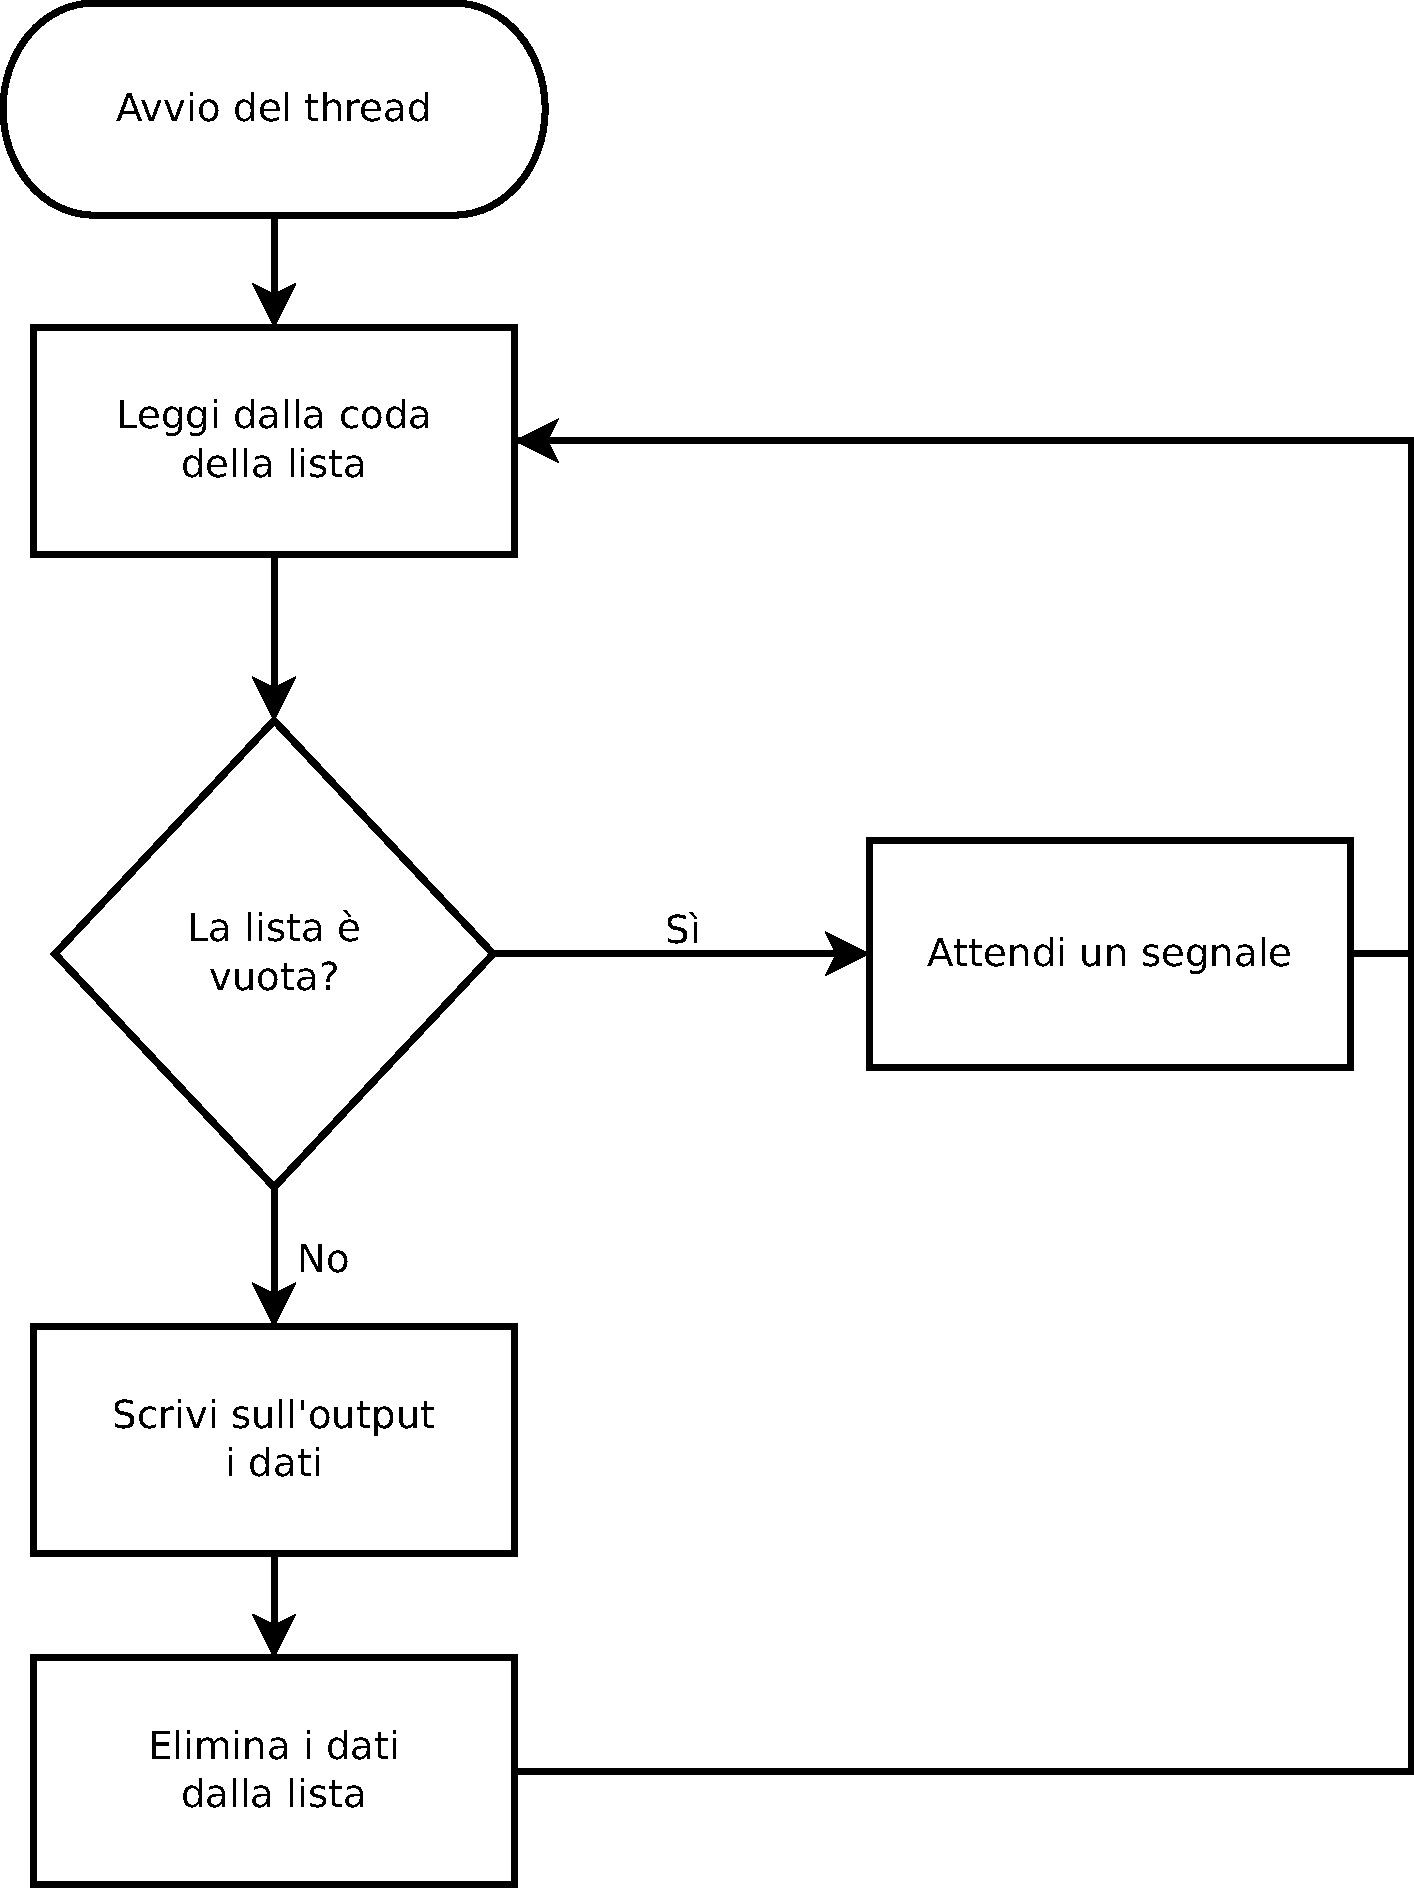
\includegraphics[width=1\linewidth]{output}
	\end{center}
	\caption{Algoritmo del thread di output}
	\label{fig:output}
\end{figure}
Il thread di output controlla i dati presenti in una lista, fornita durante
l'inizializzazione, dove verranno accodati i dati da scrivere in uscita. Quando
la lista \`e vuota, il thread si mette semplicemente in attesa, altrimenti
procede alla scrittura, rimuove dalla lista i dati scritti e ricomincia il
proprio ciclo da capo.

\subsection{Thread principale}
Avviato il thread di output, il thread principale entra nel suo ciclo
principale, dove effettua tre operazioni che esploriamo nel dettaglio:
\emph{lettura dei dati}, \emph{selezione del buffer di output} e
\emph{assegnamento al thread pool}.
\subsubsection{Lettura dei dati}
La prima operazione effettuata all'interno del ciclo principale \`e verificare
che ci sia dello spazio disponibile nel buffer circolare. Se il buffer \`e
pieno --- cio\`e se tutti i dati nel buffer devono ancora essere elaborati ---
il thread si mette in attesa che il carico di lavoro venga smaltito. Quando
c'\`e dello spazio disponibile nel buffer circolare, si leggono i dati
dall'SrcFilter e si accodano. Si procede poi alla selezione del buffer di
output.
\subsubsection{Selezione del buffer di output}
Una volta ottenuti i dati da elaborare, si verifica se esistono buffer accodati
nella lista di output. Se non ce ne sono, si crea un nuovo buffer, lo si accoda
alla lista e lo si seleziona come buffer di output; se, invece, la lista
contiene dei buffer si seleziona il buffer di testa e si verifica se \`e
utilizzabile o meno: siccome allo scopo di attutire il rumore di fondo in un
segnale spesso di fanno le somme di diversi segnali trasformati, esiste un
parametro che determina quante di queste somme si vogliono effettuare. Per ogni
buffer si tiene traccia del numero di thread a cui \`e stato assegnato e se
questo numero \`e minore rispetto al numero di somme desiderate, il buffer \`e
selezionabile, altrimenti se ne crea uno nuovo e lo si accoda in lista.
\subsubsection{Assegnamento al thread pool}
Dopo aver letto i dati del segnale da trasformare ed aver individuato il buffer
di output su cui scrivere i dati elaborati, si può assegnare il lavoro al thread
pool. Per farlo, \`e sufficiente indicare i puntatori ai due buffer ed un
puntatore alla funzione che deve occuparsi di elaborare i dati. Il thread pool
si occuper\`a automaticamente di assegnare il lavoro al primo thread libero
presente nel suo pool.
